% !TEX root = ../Dokumentation.tex
\subsection{Bilderzeugung}
\textbf{Umsetzung}\\[0.2cm]
Die Bilderzeugung ist als eigener Thread realisiert und stellt die Schnittstelle zur Kamera sicher. Die erzeugten Bilder werden fortlaufend in einer von OpenCV zu Verfügung gestellten Datenstruktur \code{cv::Mat} gespeichert, um 50\% verkleinert und über die  Methode \code{GetImage()} zu Verfügung gestellt. Die \code{GetImage()}-Methode ist dabei mittels Mutual Exclusion Threadsicher realisiert um Zugriffskonflikte zu vermeiden. Gestartet wird der Prozess automatisch bei der Objekterzeugung im Konstruktor und kann über die Methode \code{StopRecording()} angehalten werden, sobald das Programm beendet werden soll. Dem Konstruktor wird als Übergabeparameter der Pointer auf den \code{PrenController} mitgegeben, so dass im Störungsfall entsprechende Meldungen an den Controller übergeben werden können.\\
Die Raspberry Pi CAM (Abbildung \ref{fig:camera}) ist über eine MIPI Schnittstelle direkt an den Minicomputer angeschlossen liefert, mit den minimalen Auflösungseinstellungen von 640x320 Pixel, 90 Bilder pro Sekunde. Die Kamera ist über einen Servo drehbar auf einer Höhe von 170mm (Okular) montiert. Zum Schutz der Kamera dient ein Kunststoffgehäuse. 
\begin{figure}[H]
\centering
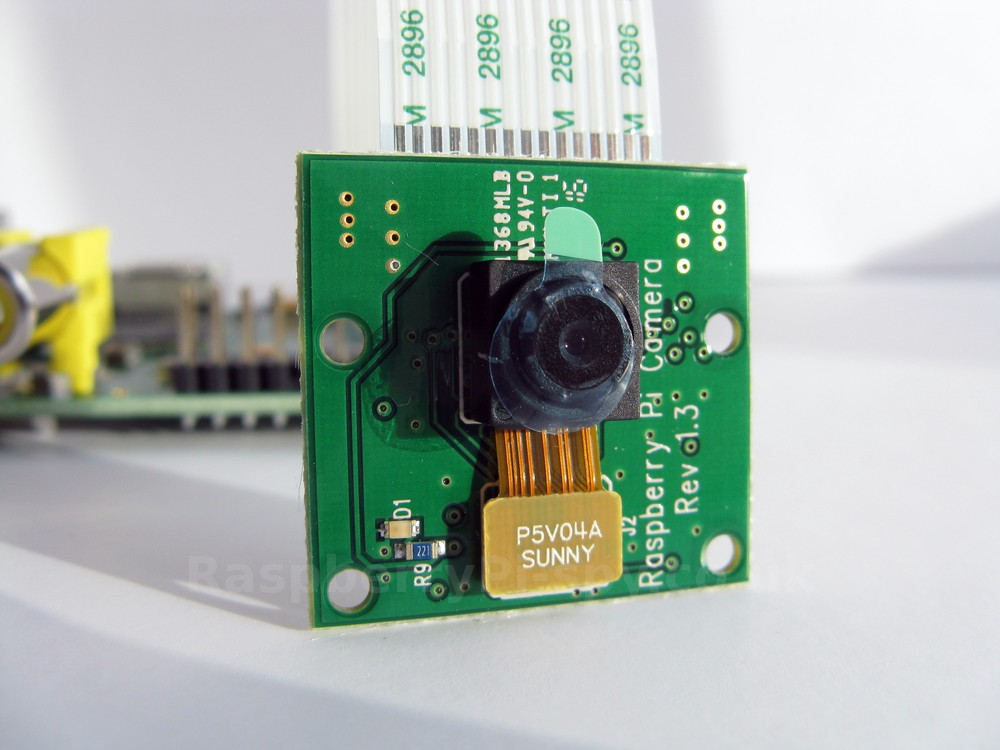
\includegraphics[width=0.6\textwidth]{03_Loesungskonzept/pictures/raspberry-pi-camera-module.jpg}
\caption{Raspberry Pi Kameramudul}
\label{fig:camera}
\end{figure}
\textbf{Vergleich Konzept und Umsetzung}\\[0.2cm]
Die Bilderzeugung ist nahezu gleich realisiert wie geplant. Einzige Unterschiede sind der Rückgabetyp, welcher von Pointer auf \code{cv::Mat} geändert worden ist und die zusätzliche Verkleinerung des Bildes um 50\%. Die Änderung des Rückgabetyps hat, gemeinsam mit der Threadsicheren Rückgabe des Bildes, die Fehlerquelle verkleinert. Die Reduktion der Auflösung hat die Rechenzeit der Fahrbahn- und Objekterkennung massiv verkleinert.\\[0.2cm]
\textbf{Bewertung}\\[0.2cm]
Die Lösung der Bilderzeugung bietet eine möglichkeit, an mehrere Prozesse Bilder schnell und zuverlässig zu Verfügung zu stellen. Die Realisierung als eigener Thread ermöglicht es dabei, Mehrkernprozessoren optimal zu nutzen. Die drehbare Kamera ermöglicht es, auf veränderte Anforderungen der Blickrichtung zu reagieren. Allerdings ist der Winkel mit 53° sehr klein. Ein Kamerasystem mit grösserem Bildwinkel wäre somit zu bevorzugen.